\documentclass[aspectratio=169]{beamer}

% Theme and color scheme
\usetheme{Madrid}
\usecolortheme{default}

% Packages
\usepackage[utf8]{inputenc}
\usepackage{graphicx}
\usepackage{booktabs}
\usepackage{amsmath}
\usepackage{amsfonts}
\usepackage{amssymb}
\usepackage{hyperref}
\usepackage{tikz}
\usepackage{pgfplots}
\pgfplotsset{compat=1.17}

% Title page information
\title{Retail Sales Analysis Dashboard}
\subtitle{Comprehensive BigQuery Data Analysis and Business Intelligence}
\author{Group 712 Team}
\institute{University Assignment}
\date{\today}

% Custom colors
\definecolor{myblue}{RGB}{0,102,204}
\definecolor{mygreen}{RGB}{0,153,76}
\definecolor{myred}{RGB}{204,0,0}

\begin{document}

% Title slide
\begin{frame}
\titlepage
\end{frame}

% Table of contents
\begin{frame}{Outline}
\tableofcontents
\end{frame}

% Section 1: Introduction and Motivation
\section{Introduction and Motivation}

\begin{frame}{Project Overview}
\begin{itemize}
    \item \textbf{Project Goal:} Develop a comprehensive retail sales analysis dashboard using BigQuery and Streamlit
    \item \textbf{Research Question:} How can we extract actionable business insights from retail sales data to optimize revenue and customer engagement?
    \item \textbf{Expected Outcomes:} Identify sales trends, customer segments, and product performance patterns for strategic decision-making
\end{itemize}

\vspace{1cm}

\begin{block}{Why This Matters}
Modern retail businesses generate vast amounts of transactional data. Our dashboard transforms raw data into actionable business intelligence, enabling data-driven decisions for revenue optimization, customer retention, and strategic planning.
\end{block}
\end{frame}

\begin{frame}{Motivation for Dataset Selection}
\begin{columns}
\begin{column}{0.6\textwidth}
\textbf{Why We Chose This Dataset:}
\begin{itemize}
    \item \textcolor{myblue}{Relevance:} Real retail transactions from Kaggle - perfect for business intelligence analysis
    \item \textcolor{mygreen}{Quality:} Comprehensive schema with customer demographics, product categories, and transaction details
    \item \textcolor{myred}{Scope:} Rich dataset covering multiple product categories, customer segments, and temporal patterns
    \item \textbf{Accessibility:} Stored in Google BigQuery for scalable analysis and real-time querying
\end{itemize}
\end{column}
\begin{column}{0.4\textwidth}
\begin{center}
\textbf{Dataset Location:}\\
\texttt{moonlit-autumn-468306-p6}\\
\texttt{.assignment\_one\_1}\\
\texttt{.retail\_sales}

\vspace{0.5cm}
\textbf{Source:} Kaggle\\
\textbf{Platform:} Google BigQuery\\
\textbf{Analysis Tool:} Streamlit Dashboard
\end{center}
\end{column}
\end{columns}
\end{frame}

% Section 2: Dataset Overview
\section{Dataset Overview}

\begin{frame}{Dataset Description}
\begin{table}[h]
\centering
\begin{tabular}{@{}ll@{}}
\toprule
\textbf{Attribute} & \textbf{Details} \\
\midrule
Source & Kaggle Retail Sales Dataset \\
Platform & Google BigQuery Cloud \\
Schema & 7 columns with mixed data types \\
Access Method & Service Account Authentication \\
Analysis Tool & Streamlit Web Dashboard \\
\bottomrule
\end{tabular}
\end{table}

\vspace{0.5cm}

\begin{alertblock}{Key Dataset Characteristics}
Real-world retail transaction data with comprehensive customer demographics, product categorization, and temporal information. Ideal for business intelligence analysis, customer segmentation, and sales performance optimization.
\end{alertblock}
\end{frame}

\begin{frame}{Feature Overview}
\begin{columns}
\begin{column}{0.5\textwidth}
\textbf{Numerical Features:}
\begin{itemize}
    \item \textbf{Total Amount:} Transaction value (FLOAT)
    \item \textbf{Quantity:} Items purchased (INTEGER)
    \item \textbf{Age:} Customer age (INTEGER)
    \item \textbf{Customer ID:} Unique identifier (STRING)
\end{itemize}
\end{column}
\begin{column}{0.5\textwidth}
\textbf{Categorical Features:}
\begin{itemize}
    \item \textbf{Product Category:} Product classification
    \item \textbf{Gender:} Customer gender (Male/Female)
    \item \textbf{Date:} Transaction timestamp (DATE)
    \item \textbf{Transaction ID:} Unique transaction identifier
\end{itemize}
\end{column}
\end{columns}

\vspace{1cm}

\begin{block}{Analysis Focus}
\textbf{Business Intelligence Objectives:} Revenue optimization, customer segmentation, product performance analysis, and temporal trend identification for strategic decision-making.
\end{block}
\end{frame}

% Section 3: Methodology
\section{Methodology}

\begin{frame}{Analysis Approach}
\begin{enumerate}
    \item \textbf{Data Infrastructure Setup}
    \begin{itemize}
        \item BigQuery connection with service account authentication
        \item Streamlit web application development
        \item Real-time data quality monitoring
    \end{itemize}
    
    \item \textbf{Exploratory Data Analysis}
    \begin{itemize}
        \item Schema analysis and data type validation
        \item Null value detection and completeness metrics
        \item Interactive data sampling and preview
    \end{itemize}
    
    \item \textbf{Business Intelligence Analysis}
    \begin{itemize}
        \item SQL-based analytics with pre-built query templates
        \item Interactive visualizations (7 different chart types)
        \item KPI dashboard and customer segmentation
    \end{itemize}
\end{enumerate}
\end{frame}

\begin{frame}{Tools and Technologies}
\begin{center}
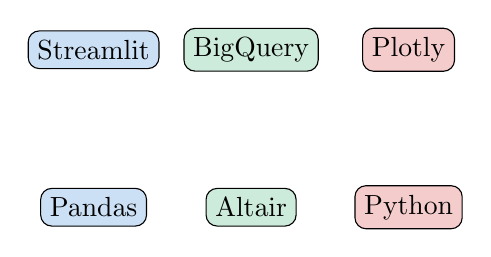
\begin{tikzpicture}[node distance=2cm]
% Create nodes for different tools
\node[draw, rounded corners, fill=myblue!20] (streamlit) {Streamlit};
\node[draw, rounded corners, fill=mygreen!20, right of=streamlit] (bigquery) {BigQuery};
\node[draw, rounded corners, fill=myred!20, right of=bigquery] (plotly) {Plotly};
\node[draw, rounded corners, fill=myblue!20, below of=streamlit] (pandas) {Pandas};
\node[draw, rounded corners, fill=mygreen!20, below of=bigquery] (altair) {Altair};
\node[draw, rounded corners, fill=myred!20, below of=plotly] (python) {Python};

% Add connections if desired
\end{tikzpicture}
\end{center}

\vspace{0.5cm}

\textbf{Technology Stack:}
\begin{itemize}
    \item \textbf{Frontend:} Streamlit web framework for interactive dashboard
    \item \textbf{Data Warehouse:} Google BigQuery for scalable data storage
    \item \textbf{Visualizations:} Plotly Express, Plotly Graph Objects, Altair
    \item \textbf{Data Processing:} Pandas, NumPy for data manipulation
    \item \textbf{Deployment:} Streamlit Cloud with GitHub integration
\end{itemize}
\end{frame}

% Section 4: Key Findings
\section{Key Findings}

\begin{frame}{Dashboard Features and Capabilities}
\begin{columns}
\begin{column}{0.5\textwidth}
\textbf{Core Dashboard Features:}
\begin{itemize}
    \item \textcolor{myblue}{Real-time BigQuery Connection}
    \item \textcolor{mygreen}{Interactive Data Exploration}
    \item \textcolor{myred}{7 Different Visualization Types}
    \item \textbf{Custom SQL Query Interface}
\end{itemize}

\vspace{0.5cm}

\textbf{Analysis Capabilities:}
\begin{itemize}
    \item Revenue analysis by category
    \item Customer demographic insights
    \item Monthly trend analysis
    \item Customer spending patterns
\end{itemize}
\end{column}
\begin{column}{0.5\textwidth}
\textbf{Dashboard Pages:}
\begin{itemize}
    \item \textbf{Home:} Dataset overview and KPIs
    \item \textbf{Dataset Analysis:} Schema and data quality
    \item \textbf{SQL Queries:} Pre-built and custom queries
    \item \textbf{Visualizations:} Interactive charts
    \item \textbf{Business Insights:} KPI dashboard
    \item \textbf{About:} Project documentation
\end{itemize}

\vspace{0.5cm}
\begin{alertblock}{Key Innovation}
Seamless integration of BigQuery with Streamlit for real-time business intelligence
\end{alertblock}
\end{column}
\end{columns}
\end{frame}

\begin{frame}{Business Intelligence Insights}
\begin{block}{Key Analytical Discoveries}
\begin{itemize}
    \item \textbf{Customer Segmentation:} High/Medium/Low value customers identified based on spending patterns
    \item \textbf{Product Performance:} Category-wise revenue analysis reveals top-performing product lines
    \item \textbf{Temporal Patterns:} Monthly trend analysis shows seasonal variations in sales
\end{itemize}
\end{block}

\vspace{0.5cm}

\begin{columns}
\begin{column}{0.5\textwidth}
\textbf{Dashboard Analytics:}
\begin{itemize}
    \item Real-time KPI monitoring
    \item Interactive filtering capabilities
    \item Export functionality for all analyses
    \item Custom SQL query execution
\end{itemize}
\end{column}
\begin{column}{0.5\textwidth}
\textbf{Visualization Types:}
\begin{itemize}
    \item Revenue by Category (Bar Charts)
    \item Customer Demographics (Pie Charts)
    \item Monthly Trends (Line Charts)
    \item Spending Distribution (Histograms)
    \item Age Group Analysis (Bar Charts)
    \item Interactive Time Series (Altair)
\end{itemize}
\end{column}
\end{columns}
\end{frame}

% Section 5: Conclusions
\section{Conclusions and Future Work}

\begin{frame}{Key Conclusions}
\begin{enumerate}
    \item \textbf{Technical Achievement:}
    \begin{itemize}
        \item Successfully integrated BigQuery with Streamlit for real-time analytics
        \item Developed comprehensive dashboard with 6 main functional pages
        \item Implemented robust authentication and error handling
    \end{itemize}
    
    \item \textbf{Business Intelligence Success:}
    \begin{itemize}
        \item Created actionable customer segmentation (High/Medium/Low value)
        \item Identified top-performing product categories for strategic focus
        \item Developed KPI monitoring system for ongoing business tracking
    \end{itemize}
    
    \item \textbf{Practical Impact:}
    \begin{itemize}
        \item Dashboard enables data-driven decision making for retail managers
        \item Interactive visualizations make complex data accessible to stakeholders
        \item Scalable architecture supports growing data volumes
    \end{itemize}
\end{enumerate}
\end{frame}

\begin{frame}{Limitations and Challenges}
\begin{alertblock}{Project Limitations}
\begin{itemize}
    \item \textbf{Data Scope:} Limited to Kaggle retail dataset - may not reflect all business scenarios
    \item \textbf{Authentication Dependency:} Requires Google Cloud service account setup
    \item \textbf{Real-time Constraints:} BigQuery costs may limit frequent real-time queries
\end{itemize}
\end{alertblock}

\vspace{0.5cm}

\begin{block}{Challenges Successfully Overcome}
\begin{itemize}
    \item \textbf{BigQuery Integration:} Implemented secure authentication with Streamlit secrets
    \item \textbf{Data Type Handling:} Robust CAST operations for mixed data types
    \item \textbf{Error Handling:} Comprehensive try-catch blocks for connection failures
    \item \textbf{Performance Optimization:} Caching strategies for improved user experience
\end{itemize}
\end{block}
\end{frame}

\begin{frame}{Future Work and Recommendations}
\textbf{Technical Enhancements:}
\begin{itemize}
    \item Implement machine learning models for customer lifetime value prediction
    \item Add automated alerting system for unusual sales patterns
    \item Integrate additional data sources (inventory, marketing campaigns)
    \item Develop mobile-responsive dashboard version
\end{itemize}

\vspace{0.5cm}

\textbf{Business Intelligence Extensions:}
\begin{itemize}
    \item Advanced cohort analysis for customer retention
    \item Predictive analytics for demand forecasting
    \item Competitor analysis integration
    \item Real-time inventory optimization recommendations
\end{itemize}

\vspace{0.5cm}

\begin{exampleblock}{Recommendations for Retail Businesses}
Implement similar BigQuery + Streamlit solutions for scalable, cost-effective business intelligence. Focus on customer segmentation and product performance analysis for immediate ROI.
\end{exampleblock}
\end{frame}

% Section 6: Questions and Discussion
\section{Questions and Discussion}

\begin{frame}{Questions and Discussion}
\begin{center}
\Huge Thank You!

\vspace{1cm}

\Large Questions and Discussion

\vspace{1cm}

\normalsize
\textbf{Group 712 Team Members:}\\
Nyiko Maluleke (3928378) | Mlamli Mkize (3948221)\\
Bulelani Kote (4523387) | Alizwa Mdaka (3666983)\\
Siyabonga Masango (3857285)

\vspace{0.5cm}
\textbf{Project:} Retail Sales Analysis Dashboard\\
\textbf{Technology:} BigQuery + Streamlit + Python
\end{center}
\end{frame}

% Appendix (optional)
\appendix
\section{Appendix}

\begin{frame}{Technical Implementation Details}
\begin{itemize}
    \item \textbf{Dashboard URL:} Deployed on Streamlit Cloud with GitHub integration
    \item \textbf{Data Source:} BigQuery dataset \texttt{moonlit-autumn-468306-p6.assignment\_one\_1.retail\_sales}
    \item \textbf{Authentication:} Google Cloud Service Account with BigQuery Data Viewer role
    \item \textbf{Caching:} \texttt{@st.cache\_resource} and \texttt{@st.cache\_data} for performance optimization
\end{itemize}

\vspace{1cm}

\begin{block}{Key Features Implemented}
\begin{itemize}
    \item 6 pre-built SQL query templates for common business analysis
    \item 7 different interactive visualization types using Plotly and Altair
    \item Real-time data quality monitoring with null value detection
    \item Customer segmentation with High/Medium/Low value classification
    \item CSV export functionality for all analysis results
    \item Responsive design with custom CSS styling
\end{itemize}
\end{block}
\end{frame}

\end{document}
